\documentclass{standalone}
\usepackage{amsmath, amssymb, amsthm}
\usepackage[usenames, dvipsnames, table] {xcolor}
\usepackage{tikz} \usetikzlibrary{calc, arrows.meta, intersections, patterns, positioning, shapes.multipart} 	% Figure

%% !TEX root = ThesisManuscript_SJ.tex
%%
%%
%%	COLORS
%%_______________________________________________
\definecolor{MyBlue}{RGB}{0,120,155}
\definecolor{MyDarkBlue}{rgb}{0, 0.25, 0.45}
\definecolor{MyBrown}{rgb}{0.28, 0.20, 0.20}
\definecolor{MyOrange}{RGB}{255,80,30}
\definecolor{MyOldOrange}{rgb}{0.75, 0.25, 0.0}
\definecolor{MyRed}{RGB}{200,0,0}
\definecolor{MyGray}{RGB}{200,200,200}
\definecolor{MyGreen}{rgb}{0.33, 0.5, 0.18}
\definecolor{MyDarkGreen}{rgb}{0.15, 0.25, 0.18}
\definecolor{MyTurquoise}{rgb}{0, 0.4, 0.4}
\definecolor{MyViolet}{rgb}{0.44, 0.16, 0.39}
\definecolor{MyYellow}{rgb}{1, 0.65, 0}

	\tikzstyle{arrow} = [->, draw=black, minimum height=0cm, outer sep=5pt, font=\small, text=black]
	\tikzstyle{enterexit} = [minimum height=0cm, text width=0.1cm, text=white, draw=none]
		
	\tikzstyle{H} = [text width=1.5cm, text=black, fill=MyGray]	

\begin{document}
\large
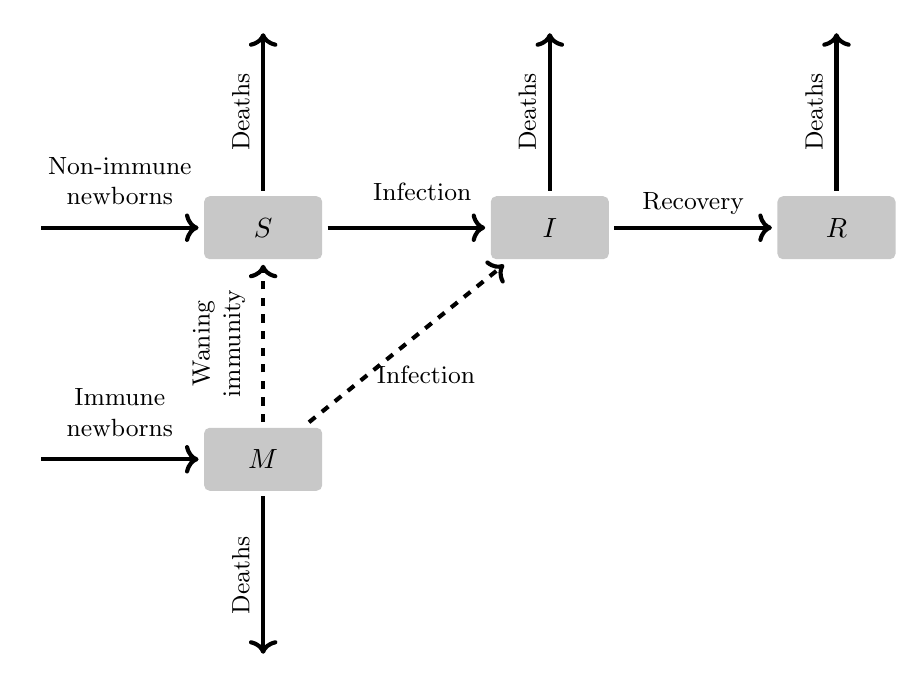
\begin{tikzpicture}[rectangle, rounded corners=2pt, node distance=2.0cm, text centered, minimum height=0.8cm, outer sep=2pt, inner sep=0pt, line width=1.5pt, draw=black]
	% HIGH
	\node (S) [H] {$S$};
	\node (M) [below = of S, H] {$M$};
	\node (I) [right= of S, H] {$I$};
	\node (R) [right = of I, H] {$R$};

	\node (enterS) [left = of S, enterexit] {};
	\node (enterM) [left = of M, enterexit] {};
	
	\node (exitS) [above = of S, enterexit] {};
	\node (exitI) [above = of I, enterexit] {};
	\node (exitR) [above = of R, enterexit] {};
	\node (exitM) [below = of M, enterexit] {};

	\draw [arrow] (enterS)  -- node[anchor=south] {\begin{tabular}{c} Non-immune \\ newborns \end{tabular} }  (S);
	\draw [arrow] (enterM)  -- node[anchor=south] {\begin{tabular}{c} Immune \\ newborns \end{tabular} }  (M);
%
	\draw [arrow,dashed] (M)  -- node[anchor=south, rotate=90] {\begin{tabular}{c} Waning \\ immunity \end{tabular}}  (S);
	\draw [arrow,dashed] (M)  -- node[anchor=north, pos=0.6, outer sep=14pt] {Infection}  (I);
	\draw [arrow] 		(S)  -- node[anchor=south, pos=0.6, outer sep=10pt] {Infection}  (I);
	\draw [arrow] (I)  --  node[anchor=south] {Recovery}  (R);

	\draw[arrow] (S) -- node[anchor=south, rotate=90] {Deaths} (exitS);
	\draw[arrow] (I)  -- node[anchor=south, rotate=90] {Deaths} (exitI);
	\draw[arrow] (R) -- node[anchor=south, rotate=90] {Deaths} (exitR);	
	\draw[arrow] (M) -- node[anchor=south, rotate=90] {Deaths} (exitM);				
 \end{tikzpicture}
\end{document}

